\documentclass[11pt]{article}
\usepackage{graphicx}
\usepackage{geometry}
\usepackage{float}
\usepackage{amsmath}
\usepackage{circuitikz}
\usepackage{amssymb}
\usepackage{mathtools}
\usepackage{tikz}
\usepackage{tikz-3dplot}
\usepackage{cite}
\usepackage{url}
\usetikzlibrary{arrows.meta,positioning,fit}
\DeclarePairedDelimiter{\set}{\{}{\}}

\title{Isotope Identification via Gamma Ray Spectroscopy}
\author{Spandan Suthar, Timo Peschken, and Stefan Rosu}
\date{November 18, 2025}

\geometry{margin=1in}
\setlength{\parindent}{0pt}

\begin{document}

\maketitle

\section{Introduction and Background}

During radioactive decay, unstable isotopes of elements decompose into
isotopes that are more energetically favorable (i.e., isotopes with lower
energy levels) \cite{harris}. During a decay process, isotopes randomly emit
photons with varying energy levels, which are detectable by
scintillation detectors \cite{mel, harris}. The frequency distribution of
photon energies allows
physicists to identify the isotopes that are decaying; this spectrum
is a characteristic
property of the isotope \cite{mel, harris}. This experiment aims to
use this fact to
identify an unknown isotope by identifying the emission energies
corresponding to the isotope's most frequent gamma ray emissions.

\vspace{1em}

In a scintillation detector, incoming gamma rays interact with a
crystal like NaI(Tl) via Compton scattering, full absorption, or
pair production \cite{mel, harris}. During full absorption, a gamma ray is
absorbed by
an electron in the crystal. This electron travels through the crystal,
causing secondary excitations of other electrons
\cite{harris,zwiebach}. The relaxations of these
secondary electrons produce scintillation photons, with an aggregate energy
equal to the energy of the recoil electron and thus of the original
gamma ray \cite{mel, mich, zwiebach}.

\vspace{1em}

In Compton scattering,
a gamma ray photon interacts with a loosely bound electron in the
potential well of an atom in the crystal, such as a valence electron, or with
similar electrons in materials surrounding the primary detector crystal
in the scintillation detector.
The photon is redirected at an angle $\theta$ relative to its
original direction of motion,
imparting only \textit{some} of its kinetic energy to the electron
(as opposed to
all of it, as in full absorption) \cite{harris}. If interacting with the
crystal, this recoil electron
again transfers energy to other electrons, causing
secondary photoemissions with aggregate energy equal to the energy of
the recoil electron \cite{ucsb, knoll}. In contrast, backscattering occurs
when the photon
interacts with surrounding material with scattering angles close to
$\theta = \pi$. In this case, a lower-energy photon is emitted by the
material and is absorbed by the crystal, causing a lower-energy recoil electron
to be freed \cite{ucsb}.

\vspace{1em}

In either case, a photocathode in the scintillation detector converts
the secondary photoemissions produced by a recoil electron
into a voltage
signal representing their total energy---thus
recovering the energy of the recoil electron \cite{mel, mich}.

\vspace{1em}

The resultant energy of the photon involved in the scattering process
is $E'$, given by \cite{harris, zwiebach, mich}:

\vspace{1em}

\begin{equation}
  \label{eq:compton_scattering}
  E' = \frac{E_\gamma}{1 + \frac{E_\gamma}{m_e c^2} (1 - \cos \theta)}
\end{equation}

\vspace{1em}

where $m_e$ is the mass of the electron, $c$ is the speed of light,
and $E_\gamma$ is the energy of the original gamma ray. Note that
full absorption produces the primary, higher-energy photopeak of an
isotope's gamma ray spectrum (with energy $E_\gamma$), whereas
Compton scattering produces
photoemissions caused by electrons that only partially
inherit the energy of the original gamma ray (with energy $E_\gamma - E'$)
\cite{harris, zwiebach}.

\section{Procedure}

A scintillation detector paired with a multi-channel
analyzer (MCA) is used to
obtain a frequency distribution of photon energies, in an arrangement
described in Figure
\ref{fig:apparatus}. Before an unknown
element is identified, calibration isotopes with
known emission peaks---namely,
Co-60, Ba-133, and Am-241---are first used to obtain a mapping from the MCA's
bin numbers to the bins' associated photon energies. Each calibration isotope
is placed in the detector
one by one. Channel numbers corresponding to emission peaks, along
with full-width at half-maximum (FWHM)
channel number bounds, are recorded, yielding the data in Table
\ref{tab:calibration}. A linear regression model is fit
to energy vs. channel
number data points, yielding a function from channel number to photon energy
used in later steps. Note that adjustment of the
scintillation detector's input voltage, preamplifier gain, and amplifier
gain may be necessary to place the emission spectrum within the MCA's
range; these
parameters should not be changed during and after calibration.

\begin{figure}[H]
  \centering
  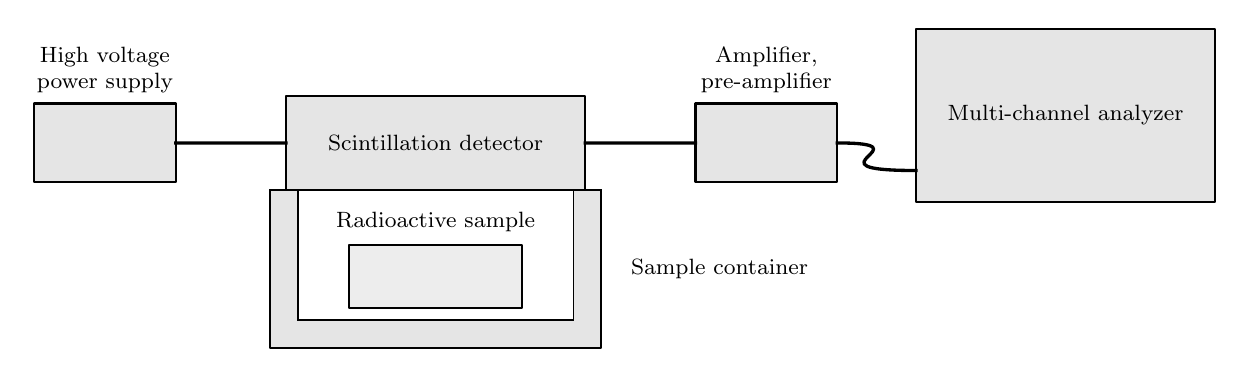
\begin{tikzpicture}[
      line cap=rect, line join=round, >=Latex,
      thick, font=\footnotesize
    ]

    % ------------------ Layout ------------------
    \def\containerWidth{4.2}
    \def\containerHeight{2.0}
    \def\wallThick{0.35}

    \def\shieldWidth{4.6}
    \def\shieldHeight{0.16}
    \def\shieldSep{0.10}

    \def\detW{3.8}
    \def\detH{1.2}
    \def\detGap{0.45}

    \def\mcaX{8.0}
    \def\mcaW{3.8}
    \def\mcaH{2.2}

    % ------------------ U-shaped container (union of three
    % rectangles + inner and outer borders) ------------------
    \fill[black!10] (-\containerWidth/2, 0) rectangle ++(\wallThick,
    \containerHeight);
    \fill[black!10] (-\containerWidth/2, 0) rectangle
    ++(\containerWidth, \wallThick);
    \fill[black!10] ( \containerWidth/2-\wallThick, 0) rectangle
    ++(\wallThick, \containerHeight);

    \draw[black, line width=0.6pt]
    (-\containerWidth/2, \containerHeight) --
    (-\containerWidth/2, 0) --
    (\containerWidth/2, 0) --
    (\containerWidth/2, \containerHeight);

    \draw[black, line width=0.6pt]
    (-\containerWidth/2+\wallThick, \wallThick) --
    (-\containerWidth/2+\wallThick, \containerHeight);
    \draw[black, line width=0.6pt]
    (\containerWidth/2-\wallThick, \wallThick) --
    (\containerWidth/2-\wallThick, \containerHeight);
    \draw[black, line width=0.6pt]
    (-\containerWidth/2+\wallThick, \wallThick) --
    (\containerWidth/2-\wallThick, \wallThick);

    \draw[black, line width=0.6pt]
    (-\containerWidth/2, \containerHeight) --
    (-\containerWidth/2+\wallThick, \containerHeight);
    \draw[black, line width=0.6pt]
    (\containerWidth/2-\wallThick, \containerHeight) --
    (\containerWidth/2, \containerHeight);

    % ------------------ Radioactive sample ------------------
    \def\sampleW{2.2}
    \def\sampleH{0.8}
    \pgfmathsetmacro{\sampleY}{\wallThick+0.15}
    \draw[fill=black!7, draw=black] (-\sampleW/2,\sampleY) rectangle
    ++(\sampleW,\sampleH);
    \node[above=1pt] at (0,\sampleY+\sampleH) {Radioactive sample};

    % ------------------ Scintillation detector ------------------
    \pgfmathsetmacro{\detY}{\containerHeight}
    \filldraw[fill=black!10, draw=black] (-\detW/2,\detY) rectangle
    ++(\detW,\detH);
    \node at (0,\detY+0.5*\detH) {Scintillation detector};

    % ------------------ High Voltage Power Supply ------------------
    \def\hvW{1.8}
    \def\hvH{1.0}
    \pgfmathsetmacro{\hvX}{-4.2}
    \pgfmathsetmacro{\hvY}{\detY + 0.1}
    \filldraw[fill=black!10, draw=black] (\hvX-\hvW/2,\hvY)
    rectangle ++(\hvW,\hvH);
    \node[above, align=center] at (\hvX,\hvY+\hvH)
    {High voltage\\power supply};

    % ------------------ Amplifier ------------------
    \def\ampW{1.8}
    \def\ampH{1.0}
    \pgfmathsetmacro{\ampX}{4.2}
    \pgfmathsetmacro{\ampY}{\detY + 0.1}
    \filldraw[fill=black!10, draw=black] (\ampX-\ampW/2,\ampY)
    rectangle ++(\ampW,\ampH);
    \node[above, align=center] at (\ampX,\ampY+\ampH)
    {Amplifier,\\pre-amplifier};

    % ------------------ MCA ------------------
    \filldraw[fill=black!10, draw=black] (\mcaX-\mcaW/2,\detY-0.15)
    rectangle ++(\mcaW,\mcaH);
    \node at (\mcaX, \detY-0.15+\mcaH/2) {Multi-channel analyzer};

    % ------------------ Signal path ------------------
    \draw[very thick]
    (\hvX+\hvW/2, \hvY+\hvH/2)
    .. controls +(1.0,0.0) and +(-1.0,0.0) ..
    (-\detW/2, \detY+0.5*\detH);

    \draw[very thick]
    (\detW/2, \detY+0.5*\detH)
    .. controls +(1.0,0.0) and +(-1.0,0.0) ..
    (\ampX-\ampW/2, \ampY+\ampH/2);

    \draw[very thick]
    (\ampX+\ampW/2, \ampY+\ampH/2)
    .. controls +(1.2,0.0) and +(-1.5,0.0) ..
    (\mcaX-\mcaW/2, \detY+0.25);

    % ------------------ Signal label ------------------
    \pgfmathsetmacro{\signalMidX}{(\detW/2 + \mcaX - \mcaW/2)/2}

    % ------------------ Helper labels ------------------
    \node[anchor=west] at (\containerWidth/2+0.25,
    \containerHeight/2) {Sample container};

  \end{tikzpicture}

  \caption{A schematic of the experimental apparatus. A radioactive
    sample is placed in a container. A scintillation detector, powered by a
    high-voltage power supply, is
    placed directly above the
    sample, collecting gamma rays and causing either full absorption
    or Compton scattering and converting the resultant secondary
    photoemissions into voltage
    signals. A pre-amplifier and amplifier pair adjust the voltage signals to
    suitable parameters for the MCA: the voltage is set to an
    expected operation range
  and voltage pulses are shaped to be well-defined on an oscilloscope.}
  \label{fig:apparatus}
\end{figure}

To verify the correctness of the calibration, a sample of Cs-137 is
placed within the detector. The emission spectrum is recorded, along
with the peak's centroid channel number and FWHM channel number
bounds, producing the data in Figure \ref{fig:cs137_spectrum}. An entirely
unknown isotope is then placed in the
detector for identification. Channel numbers of emission
peaks and FWHM bounds are again recorded, producing the data points in Table
\ref{tab:unknown}.

\begin{figure}[H]
  \centering
  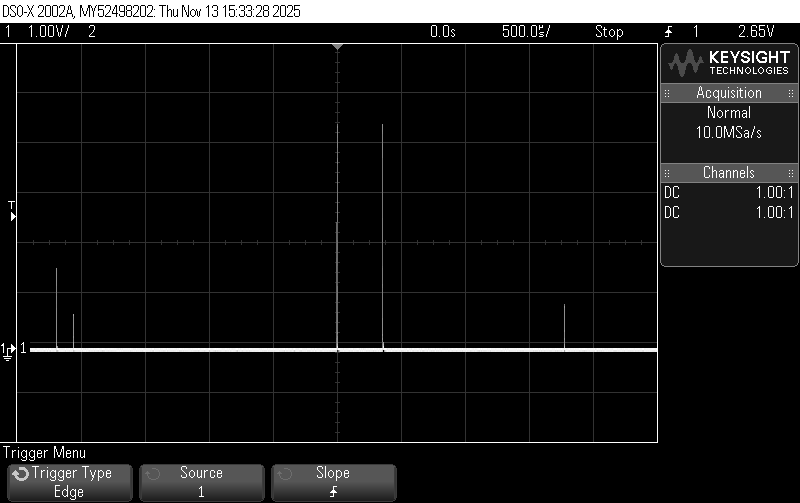
\includegraphics[width=0.9\textwidth]{osc.png}
  \caption{Voltage pulses corresponding to emission events from a
    Cs-137 sample, recorded
    on an oscilloscope monitoring the amplifier output. The heights of
    the pulses are
    proportional to the aggregate energy of the secondary
    photoemissions caused by recoil electrons from Compton scattering
    and full absorption \cite{harris}. "Darker" horizontal bands on
    the oscilloscope trace correspond to low-frequency features of the
    emission spectrum, such as the space between the Compton edge and
  the photopeak.}
  \label{fig:osc}
\end{figure}

\section{Results}

The known energies vs. channel number data points used to calibrate
the detector and MCA are presented
in Table \ref{tab:calibration}, while the linear model providing the
conversion from channel numbers to photon energies is displayed in
Figure \ref{fig:calibration}.

\begin{table}[h]
  \centering
  \begin{tabular}{lccccc}
    \hline
    Isotope & Known Energy & Channel & FWHM & Estimated Energy &
    Discrepancy \\
    & (keV) & (Index) & (Index) & (keV) & \\
    \hline
    Co-60 & 1173.0 & $790$ & $42$ & $1170 \pm 28$ & $0.11\sigma$ \\
    Co-60 & 1332.5 & $895$ & $44$ & $1326 \pm 29$ & $0.22\sigma$ \\
    Ba-133 & 302.9 & $212$ & $50$ & $310 \pm 30$ & $0.24\sigma$ \\
    Ba-133 & 356.0 & $250$ & $20$ & $364 \pm 13$ & $0.62\sigma$ \\
    Am-241 & 59.6 & $46$ & $5$ & $59 \pm 4$ & $0.15\sigma$ \\
    \hline
  \end{tabular}
  \caption{Known energies, recorded channel numbers, full-width at
    half-maximum interval widths, and estimated energies for the
    calibration isotopes
    Co-60, Ba-133, and Am-241. Note that Co-60 and Ba-133 have two
    emission peaks, while Am-241 has one. Discrepancies between
    estimated and known
  energies lie within 1$\sigma$.}
  \label{tab:calibration}
\end{table}

\begin{figure}[H]
  \centering
  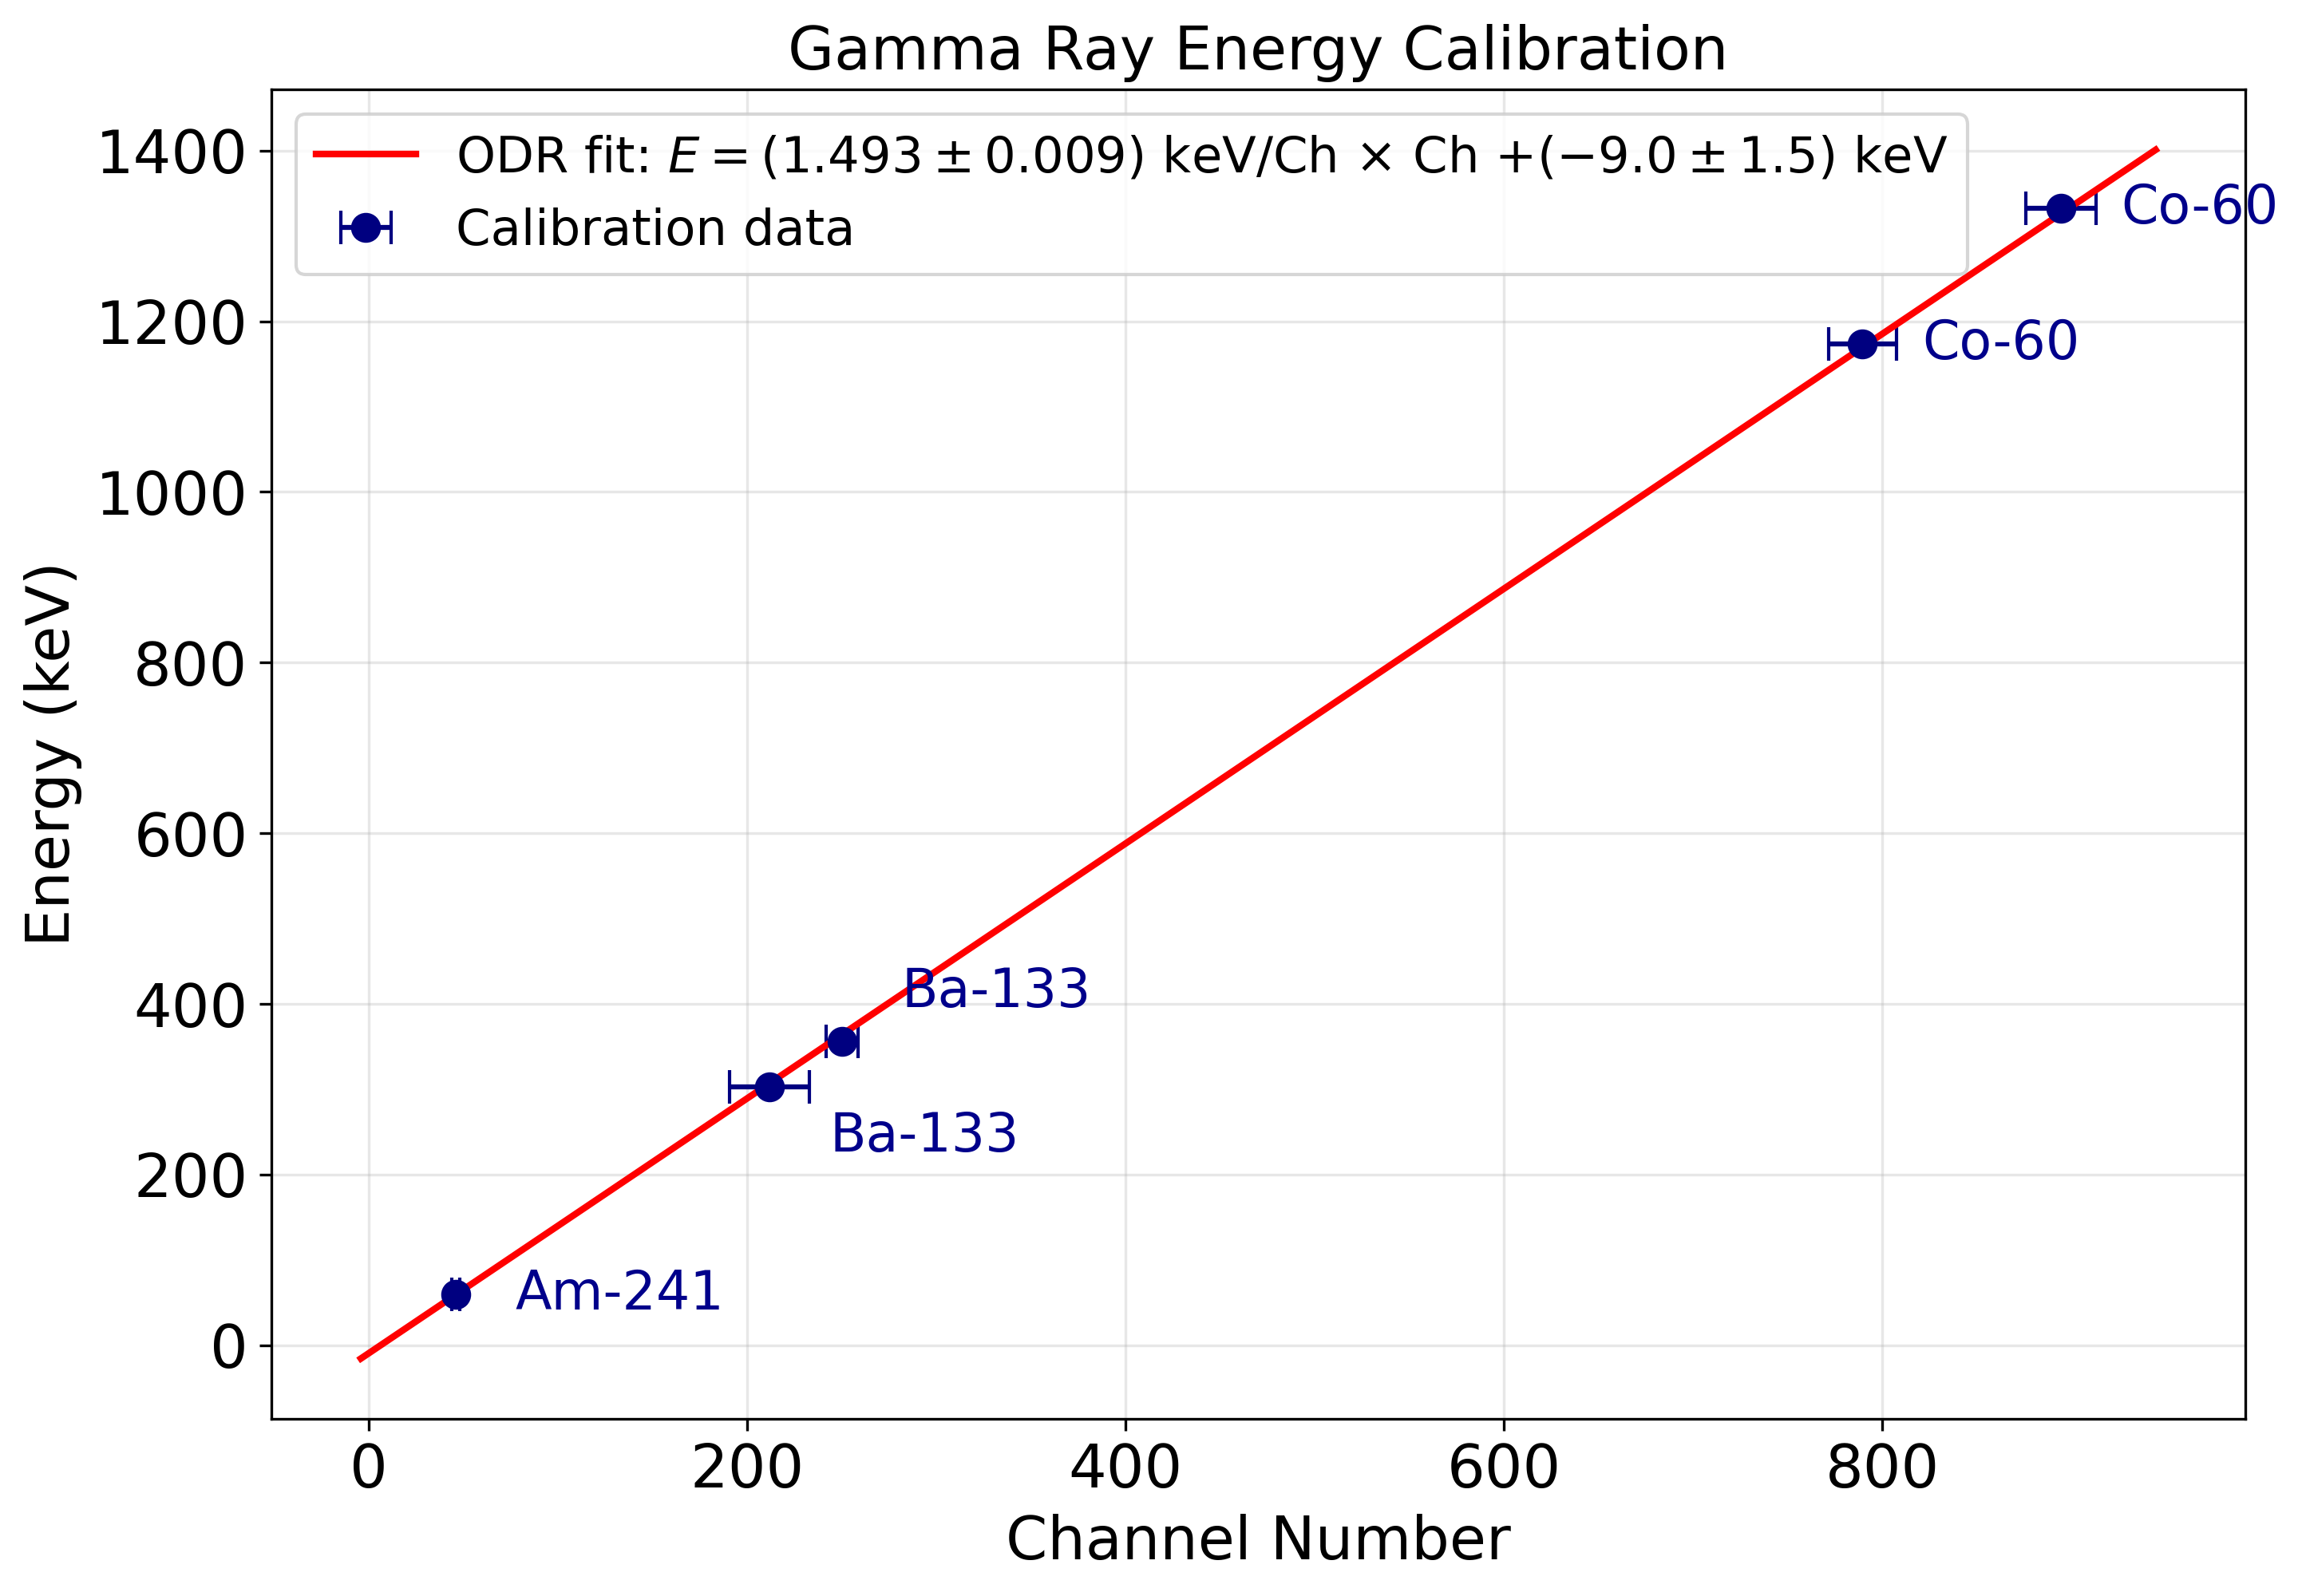
\includegraphics[width=0.8\textwidth]{calibration.png}
  \caption{Linear regression model (red) used to convert MCA channel
    numbers to photon energies, derived from known-energy vs. channel
  number data points (blue) obtained from the calibration isotopes.}
  \label{fig:calibration}
\end{figure}

Figure \ref{fig:cs137_spectrum} includes
a plot of the emission spectrum of Cs-137 with energies obtained from the
regression model. Notable features of the spectrum are identified, including
the primary photopeak, Compton backscatter peak, Compton plateau,
Compton edge,
and the X-ray photopeak. Using equation \ref{eq:compton_scattering}
with a known Cs-137 photopeak energy of $E_\gamma = 662$ keV \cite{cs137}, the
Compton backscatter peak is calculated to occur at 184.3 keV ($\theta
= \pi$), with the Compton edge occurring at 477.4 keV ($\theta = 0$)
\cite{harris}.

\begin{figure}[H]
  \centering
  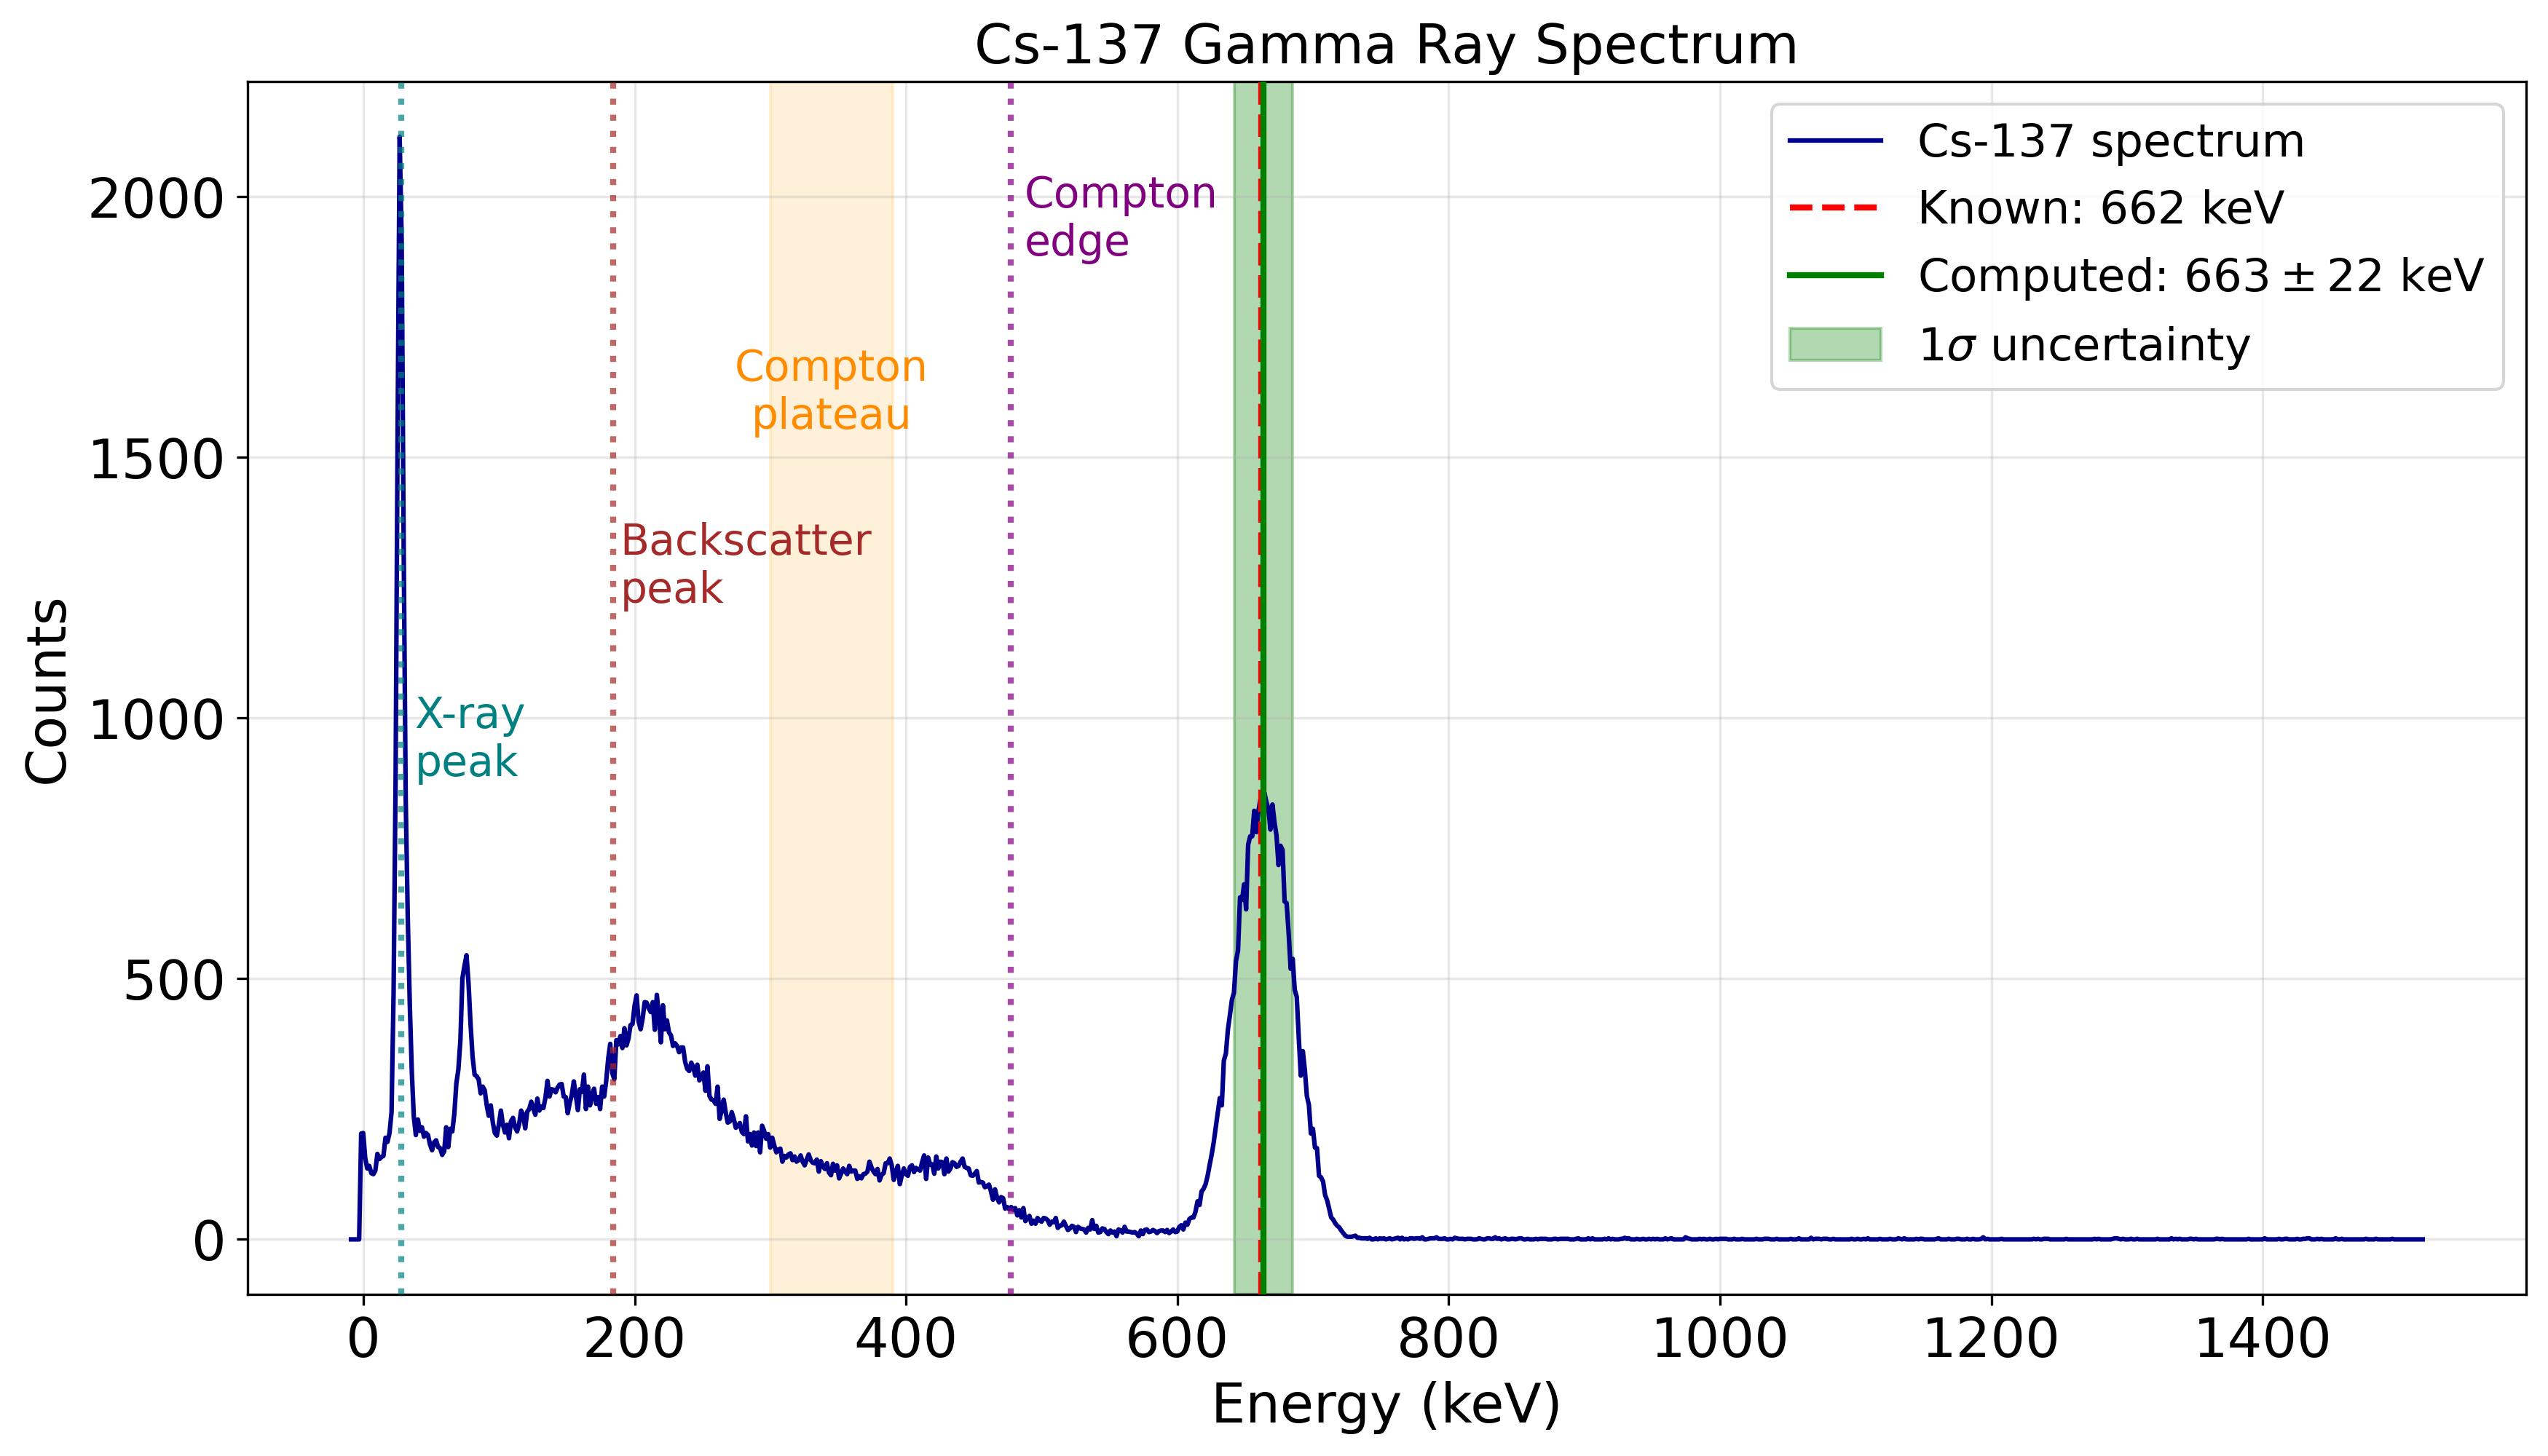
\includegraphics[width=0.9\textwidth]{cs137_spectrum.png}
  \caption{A spectrum of Cs-137 collected from the MCA, with energies
    derived from channel numbers using
    the linear regression model from Figure \ref{fig:calibration}.
    The X-ray peak (light blue), theoretical Compton
    backscatter peak (red, 184.3 keV), Compton plateau (yellow), and Compton
    edge (purple, 477.4 keV) are
    identified. The known full-absorption photopeak (red, 662 keV)
    and the computed
    full-absorption photopeak (green, 663 keV $\pm$ 22 keV) are also
  identified.}
  \label{fig:cs137_spectrum}
\end{figure}

Table \ref{tab:unknown} includes the channel numbers
and estimated energies of the unknown isotope. The emission peak
energies of the
unknown isotope are found to agree within 1$\sigma$ of the known
emission peaks of Ra-226 \cite{ra226}, strongly suggesting it is the
unknown isotope. The
computed peak energies of the unknown isotope in comparison with
Ra-226's peak energies are presented in Table \ref{tab:unknown}.

\begin{table}[h]
  \centering
  \begin{tabular}{cccc}
    \hline
    Channel & Computed Energy & Ra-226 Candidate Peak & Discrepancy \\
    (Index) & (keV) & (keV) & \\
    \hline
    $131.76$ & $188\pm 5$ & $186$ & $0.35\sigma$ \\
    $169.86$ & $244\pm 6$ & $242$ & $0.43\sigma$ \\
    $205.26$ & $297\pm 7$ & $295$ & $0.33\sigma$ \\
    $245.36$ & $357 \pm 8$ & $351$ & $0.75\sigma$ \\
    $417.46$ & $614 \pm 14$ & $609$ & $0.36\sigma$ \\
    \hline
  \end{tabular}
  \label{tab:unknown}
  \caption{Channel numbers of emission peaks of the unknown isotope,
    with computed energies
    and possible Ra-226 emission peaks \cite{ra226}. Discrepancies between the
    estimated energies and the known
  energies of Ra-226 lie within 1$\sigma$.}
\end{table}

\section{Conclusion and Discussion}

An MCA paired with a scintillation detector is found to be a reliable
tool for producing gamma ray emission spectra of radioactive
isotopes. The function from MCA channel numbers resulting from the calibration
of such a system is found to reproduce the known energies of the
calibration isotopes within 1$\sigma$ of accepted values and the
emission peak of Cs-137 to within 1$\sigma$ of the accepted value,
suggesting a successful calibration process.

\vspace{1em}

Notable features of the emission spectrum of Cs-137 are identified. The
Compton backscatter peak and Compton edge qualitatively occur near the
theoretical energies of 184.3 keV and 477.4 keV, with the Compton
plateau corresponding to a continuum of possible scattering angles
between $\theta = 0$ and
$\theta = \pi$. A backscattering peak is formed toward the
lower end of the scattering spectrum; this peak results from scattering
events corresponding to $\theta$-values between $\theta = \frac{2
\pi}{3}$ and $\theta = \pi$,
which produce a narrower spread of energies than those corresponding to
$\theta$-values between $\theta = 0$ and $\theta = \frac{2 \pi}{3}$
\cite{knoll}. Low-energy x-ray peaks are also observed near $30$ keV,
corresponding to decay events of Cs-137 into its next decay product, Ba-137,
without emitting a typical $662$ keV gamma ray. In these cases, an electron
occupying a $1s$ state is ejected from the atom,
and an electron occupying a higher-energy state within the atom relaxes to fill
the $1s$ hole, emitting the lower-energy x-ray photon \cite{ucsb, france, mel}.

\vspace{1em}

The unknown isotope investigated is identified to be Ra-226, with all computed
emission peaks agreeing within 1$\sigma$ of the corresponding known
emission peaks of Ra-226.

\bibliographystyle{plain}
\bibliography{report}

\end{document}
